\section{Exercise 4. Code multipath}
The code multipath can be seen by plotting the difference of code and carrier
ionosphere-free combinations (PC-LC). The evolution of this difference can be
followed with a sampling rate of 1 Hz. Due to its geometric nature, the effect
of multipath repeats with the receiver-satellite geometry.\\

The RINEX files \textbf{UPC33600.08N}, \textbf{UPC33610.08N}, UPC33620.08N contain
observations at 1 Hz collected by a GPS receiver with fixed coordinates over
the same period of time on three consecutive days. The corresponding
navigation files are \textbf{BRD3600.08N}, \textbf{BRD3610.08N}, \textbf{BRD3620.08N}.\\

Using gLAB, read the RINEX files, plot the combination PC-LC and identify
the effect of multipath. Analyse the measurements of satellites PRN20 and
PRN25 in the time interval 67000 < t < 68000s. Include the satellite's
elevation in the plots.\\

\subsection{Exercise 4.1 PC Code multipath}
Complete the following steps to depict the noise and multipath in the PC combination:
\begin{enumerate}
        \item Read the RINEX files, execute:
        \begin{figure}[H]
            \centering
            \begin{minted}[fontsize=\footnotesize, bgcolor=bg, breaklines, tabsize=2, frame=lines, framesep=2mm]{console}
            gLAB linux -input:cfg meas.cfg -input:obs UPC33600.08 -input:nav BRD3600.08N > upc3360.meas 
            \end{minted}
            \caption{}
            \label{}
        \end{figure}
        
        \item Verify the following field contents in the generated file upc3360.meas and others:
        
        \begin{figure}[H]
            \centering
            \begin{minted}[fontsize=\footnotesize, bgcolor=bg, breaklines, tabsize=2, frame=lines, framesep=2mm]{python}
            [Id YY Doy sec GPS PRN el Az N. list C1C L1C C1P L1P C2P L2P]
            [1 2 3 4 5 6 x x 9 10 11 xx 13 14 15 16 ]
            \end{minted}
            \caption{}
            \label{}
        \end{figure}

                
        \item Compute the difference of code and carrier ionosphere-free combinations: (i.e. apply next equation) :
\end{enumerate}
    



\begin{equation}\label{Pcode_iono-free}
P_{C} = \frac{f_{1}^{2}P_{1}-f_{2}^{2}P_{2}}{f_{1}^{2}-f_{2}^{2}}
=
\frac{\gamma P_{1}-P_{2}}{\gamma - 1}
\end{equation}

\begin{equation}\label{Carrier_iono-free}
L_{C} = \frac{f_{1}^{2}P_{1}-f_{2}^{2}P_{2}}{f_{1}^{2}-f_{2}^{2}}
=
\frac{\gamma L_{1}-L_{2}}{\gamma - 1}
\end{equation}

Where:

\begin{equation}\label{Pcode_iono-free}
M_{P_{C}} = P_{C}-L_{C}
\end{equation}

\begin{figure}[H]
            \centering
            \begin{minted}[fontsize=\footnotesize, bgcolor=bg, breaklines, tabsize=2, frame=lines, framesep=2mm]{console}
            gawk 'BEGIN{g12=(154/120)**2}{if ($4>66000 && $4<69000)
            print $6,$4,(g12*$13-$15)/(g12-1)-(g12*$14-$16)/(g12-1),$7}' upc3360.meas > upc3360.LcPc
            \end{minted}
            \caption{}
            \label{}
\end{figure}

\textbf{\textcolor{Blue}{(Similarly for the other two files upc3361.meas and upc3362.meas.)}}

Plot the results:
\begin{figure}[H]
            \centering
            \begin{minted}[fontsize=\footnotesize, bgcolor=bg, breaklines, tabsize=2, frame=lines, framesep=2mm]{console}
            graph.py -f upc3360.LcPc -c '($1==20)' -x2 -y3 -s- -l "DoY 360"
                -f upc3361.LcPc -c '($1==20)' -x2 -y3 -s- -l "DoY 361"
                -f upc3362.LcPc -c '($1==20)' -x2 -y3 -s- -l "DoY 362"
                -f upc3360.LcPc -c '($1==20)' -x2 -y4 -l "Elev (deg.)"
            \end{minted}
            \caption{}
            \label{}
\end{figure}

Repeat the same plots, but shift the plot of the second day by 3m 56s = 236s and the third day by 2x(3m 56s) = 472s

\begin{figure}[H]
            \centering
            \begin{minted}[fontsize=\footnotesize, bgcolor=bg, breaklines, tabsize=2, frame=lines, framesep=2mm]{console}
            graph.py -f upc3360.LcPc -c '($1==20)' -x2 -y3 -s- -l "DoY 360"
                -f upc3361.LcPc -c '($1==20)' -x'($2+236)' -y3 -s- -l "DoY 361"
                -f upc3362.LcPc -c '($1==20)' -x'($2+472)' -y3 -s- -l "DoY 362"
                -f upc3360.LcPc -c '($1==20)' -x2 -y4 -l "Elev (deg.)"
            \end{minted}
            \caption{}
            \label{}
\end{figure}



\begin{figure}[H]
    \centering
    \begin{subfigure}{0.45\textwidth}
        \centering
        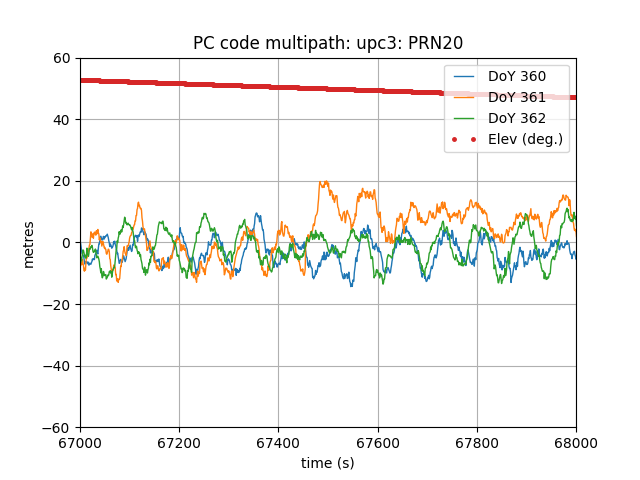
\includegraphics[scale=0.52]{sources/Figures/FIG_2/TUT2_Ex4.1a.png}
        \caption{}
        \label{fig:subfig1}
    \end{subfigure}
    \hfill
    \begin{subfigure}{0.45\textwidth}
        \centering
        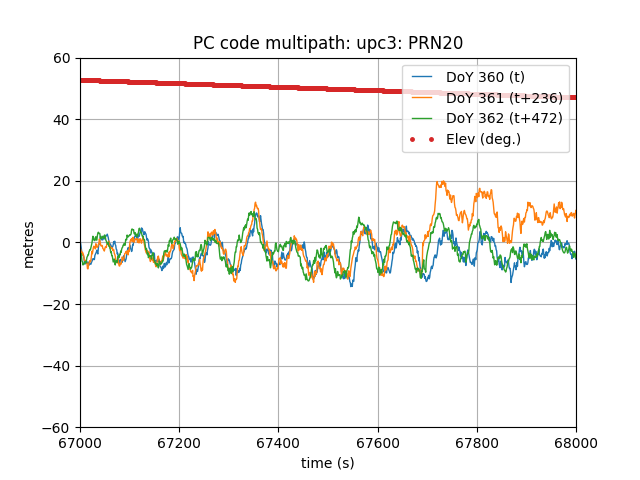
\includegraphics[scale=0.52]{sources/Figures/FIG_2/TUT2_Ex4.1b.png}
        \caption{}
        \label{fig:subfig2}
    \end{subfigure}
    \caption{}
    \label{fig:dos-figuras-juntas}
\end{figure}


\begin{figure}[H]
        \centering
        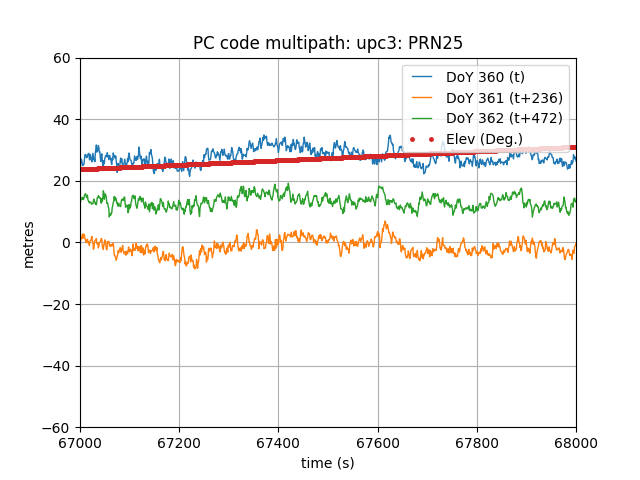
\includegraphics[scale=0.52]{sources/Figures/FIG_2/TUT2_Ex4.1.5.png}
        \caption{}
        \label{}
\end{figure}
\usepackage{subcaption}







\begin{itemize}
    \item What is the reason for the observed 3m 56s displacement between the graphs for two consecutive days?
    \item Repeat the previous plot for the satellite PRN25 and compare results.
\end{itemize}

\textcolor{Green}{OPTIONAL: Repeat the multipath analysis of the previous exercise using
files htv13450.04o, htv13460.04o, htv13470.04o collected by the
permanent receiver HTV1, and files galb3450.04o, galb13460.04o,
galb13470.04o collected by the permanent receiver GALB. The associated
broadcast orbit files are brdc3450.04n, brdc3460.04n, brdc3470.04n.}



\subsection{Exercise 4.2. Melbourne-Wübbena multipath}

Complete the following steps to depict the noise and multipath in the Melbourne Wübbena combination:

\begin{equation}\label{Pcode_Wübbena}
P_{N} = \frac{f_{1}P_{1}+f_{2}P_{2}}{f_{1}+f_{2}}
=
\frac{\sqrt{\gamma} P_{1}-P_{2}}{\sqrt{\gamma} - 1}
\end{equation}

\begin{equation}\label{Carrier_Wübbena}
L_{W} = \frac{f_{1}L_{1}-f_{2}L_{2}}{f_{1}-f_{2}}
=
\frac{\sqrt{\gamma} L_{1}-L_{2}}{\sqrt{\gamma} - 1}
\end{equation}

Where:

\begin{equation}\label{Pcode_Wübbena}
M_{MW} = P_{N}-L_{W}
\end{equation}


Execute (in a single line):\\

\begin{figure}[H]
            \centering
            \begin{minted}[fontsize=\footnotesize, bgcolor=bg, breaklines, tabsize=2, frame=lines, framesep=2mm]{console}
            gawk 'BEGIN{s12=154/120}{print $6,$4,(s12*$14-$16)/(s12-1)-(s12*$13+$15)/(s12+1),$7}' galb3450.meas > galb3450.MW
            \end{minted}
            \caption{}
            \label{}
\end{figure}


\textbf{\textcolor{Blue}{(Similarly for the other files)}}\\

And plot results.





\subsection{Exercise 4.3. C1 code multipath}
The C1 code multipath and receiver noise can be depicted using the following combination (that removes all frequency dependent and not dependent terms):

\begin{equation}\label{}
M_{C_{1}} =C_{1}-L_{1}-2\alpha\left(L_{1}-L_{2}\right) ; \ \ \ \ \ \ \alpha = \frac{f_{2}^{2}}{f_{1}^{2}-f_{2}^{2}} = \frac{1}{\gamma -1} = 1.545 ; \ \ \ \ \ \ \gamma = \left(\frac{77}{60}\right)^{2}
\end{equation}


\begin{itemize}
    \item \textbf{\textcolor{Blue}{Generate the “meas” file: Select, for instance, PRN03}}
    \begin{figure}[H]
            \centering
            \begin{minted}[fontsize=\footnotesize, bgcolor=bg, breaklines, tabsize=2, frame=lines, framesep=2mm]{console}
            gLAB_linux -input:cfg meas.cfg -input:obs UPC33510.08O|gawk '{if ($6==03)print $0}'>upc3.meas
            \end{minted}
            \caption{}
            \label{}
    \end{figure}
    \begin{figure}[H]
            \centering
            \begin{minted}[fontsize=\footnotesize, bgcolor=bg, breaklines, tabsize=2, frame=lines, framesep=2mm]{python}
            [Id YY Doy sec GPS PRN el Az N. list C1C L1C C1P L1P C2P L2P]
            [1 2 3 4 5 6 7 8 9 10 11 12 13 14 15 16 ]
            \end{minted}
            \caption{}
            \label{}
    \end{figure}

    
    \item \textbf{\textcolor{Blue}{Using previous expression, compute the C1 multipath and code noise:}}
    \begin{figure}[H]
            \centering
            \begin{minted}[fontsize=\footnotesize, bgcolor=bg, breaklines, tabsize=2, frame=lines, framesep=2mm]{console}
            gawk '{print $4,$11-$14-3.09*($14-$16)-21.3}' upc3.meas> upc3.C1
            \end{minted}
            \caption{}
            \label{}
    \end{figure}


    
    \item \textbf{\textcolor{Blue}{Plot results for PRN03:}}
    \begin{figure}[H]
            \centering
            \begin{minted}[fontsize=\footnotesize, bgcolor=bg, breaklines, tabsize=2, frame=lines, framesep=2mm]{console}
            graph.py -f upc3.C1 -s- --l "C1 Raw" --xn 35000 --xx 40000  --yn -5 --yx 5 --xl "time (s)" --yl "meters"  -t "PRN03, C1 Raw measurement noise and multipath"
            \end{minted}
            \caption{}
            \label{}
    \end{figure}
\end{itemize}



